\documentclass{beamer}
\usetheme{Madrid}
\usecolortheme{crane}
\usepackage{animate}
\usepackage{graphicx}
\usepackage{amsmath}
\usepackage{amsfonts}
\usepackage{amssymb}
\usepackage{amsthm}
\usepackage{complexity}
\usepackage{caption}
% \usepackage{subcaption}
\usepackage{enumerate}
\usepackage{enumitem}
\usepackage{array}   % for \newcolumntype macro
% \usepackage{refcheck}
\newcolumntype{L}{>{$}l<{$}} % math-mode version of "l" column type
\newcolumntype{R}{>{$}r<{$}} % math-mode version of "r" column type
\newcolumntype{C}{>{$}c<{$}} % math-mode version of "c" column type
% %%%theoerms, etc%%%%
% \theoremstyle{plain}% default
% \newtheorem{thm}{Theorem}
% \newtheorem{prop}{Proposition}
% \newtheorem{pf}{Proof}
% \newtheorem{lem}{Lemma}
% \theoremstyle{definition}
% \newtheorem{definition}{Definition}
% \newtheorem{example}{Example}
% \theoremstyle{remark}
% \newtheorem{rmk}{Remark}
% \newtheorem{case}{Case}
% \newtheorem{prob}{Problem}
% \newtheorem{observation}{Observation}

%%%%%%%%custom commands
\newcommand{\ith}{i^\text{th}}
\newcommand{\jth}{j^\text{th}}
\newcommand{\kth}{k^\text{th}}
\newcommand{\NN}{\mathbb{N}} %  set of natural numbers
\newcommand{\ZZ}{\mathbb{Z}} %  set of integer number
\newcommand{\RR}{\mathbb{R}} %  set of real numbers
\newcommand{\SH}{\mathbb{S}} %  set of unit vectors
\newcommand{\HH}{{\mathcal{H}}} %  Calligraphic H
\renewcommand{\PP}{{\mathcal{P}}} %  Calligraphic P
\newcommand{\DD}{{\mathcal{D}}} %  Calligraphic D
\newcommand{\QQ}{{\mathcal{Q}}} %  Calligraphic D
\newcommand{\FF}{{\mathcal{F}}} %  Calligraphic D
\newcommand{\bbH}{{\mathbb{H}}}
\newcommand{\bbR}{{\mathbb{R}}}
\newcommand{\bbP}{{\mathbb{P}}}
\newcommand{\bbZ}{{\mathbb{Z}}}
\newcommand{\bbC}{{\mathbb{C}}}
\newcommand{\bbQ}{{\mathbb{Q}}}
\newcommand{\bbA}{{\mathbb{A}}}
\newcommand{\bbF}{{\mathbb{F}}}
\newcommand{\bbh}{{\mathbb{H}}}
\newcommand{\bbr}{{\mathbb{R}}}
\newcommand{\bbp}{{\mathbb{P}}}
\newcommand{\bbz}{{\mathbb{Z}}}
\newcommand{\bbc}{{\mathbb{C}}}
\newcommand{\bbq}{{\mathbb{Q}}}
\newcommand{\bba}{{\mathbb{A}}}
\newcommand{\bbf}{{\mathbb{F}}}
\newcommand{\bbn}{{\mathbb{N}}}
\newcommand{\bbN}{{\mathbb{N}}}

\title[Protein Folding]
{Protein Folding}
\subtitle{Planar Configuration Spaces of Disk Arrangements and
Hinged Polygons}
\author{Clinton Bowen}
\institute
{
  California State University Northridge
}
\date
{December 6, 2016}
\subject{Mathematics}
\begin{document}
\frame{\titlepage}
\section{Motivation}

% A long standing problem in molecular biology is to determine the three dimensional structure of a protein when only given the sequence of amino acid residues which comp ose the protein chain  Due to the complexity of the protein folding problem  scientists have prop osed a variety of mo dels which attempt to simplify the problem by abstracting only the  essential physical prop erties  of real proteins  In these mo dels  the three dimensional space is often represented by a lattice  Residues which are adjacent in the primary sequence  i e  covalently linked  must b e placed at adjacent p oints in the lattice  A conformation of a protein is simply a self avoiding walk along the lattice  The protein folding problem STRING FOLD is that of  nding a conformation of the protein sequence on the lattice such that the overall energy is minimized  for some reasonable de nition of energy  The lattice formulation describ ed so far leaves op en two imp ortant questions  what typ e of lattice should one use  and what energy function is appropriate  Once these two questions have b een answered  one may then address the algorithmic complexity of optimizing the energy function for the lattice 
% For a variety of such In this pap er  we
% simple mo dels  this minimization problem is in fact NP hard               consider the Hydrophobic Polar  HP  Model intro duced by Dill      The HP
% proteins into two For concreteness  we will take our input to b e a  nite string over the alphab et fH  Pg    where P represents p olar residues  and H represents hydrophobic residues  Dill et al      survey the literature analyzing this
% mo del 
  \begin{frame}
  % Protein folding is the physical process by which a protein chain acquires its native 3-dimensional structure, a conformation that is usually biologically functional, in an expeditious and reproducible manner.
    \frametitle{Protein Folding}
    Protein folding is the process in which a protein chain acquires its 3-dimensional structure.
    \begin{columns}[c] % the "c" option specifies center vertical alignment
    \column{.5\textwidth} % column designated by a command
     \begin{itemize}
     	\item[*] Proteins in an organism fold into a specific geometric pattern (sometimes referred as its \textit{native state}).
     	\item[*]  Geometric patterns can determine a protein's function and behavior. 
     \end{itemize}
    \column{.5\textwidth}
	     \begin{minipage}{\linewidth}
			\begin{center}
			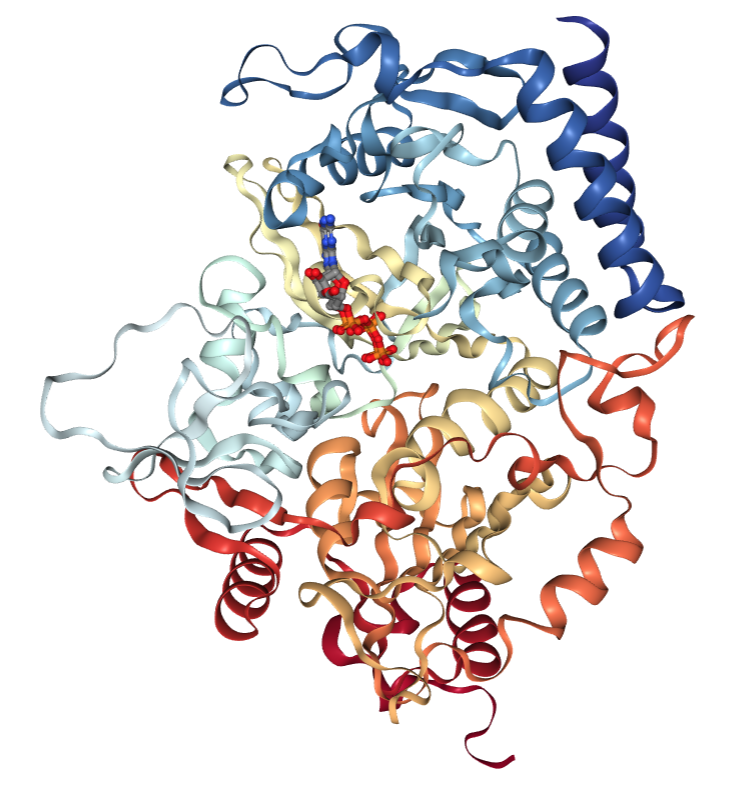
\includegraphics[width=.66\columnwidth]{graphics/5FH3.png}
			\captionof{figure}{
The structure of rat cytosolic PEPCK variant E89A in complex with oxalic acid and GTP \cite{Rats}.}
			\end{center}
		\end{minipage}
    \end{columns}
  \end{frame}

  \begin{frame}
    \frametitle{Hinged Dissections}
     \begin{columns}[c] 
    \column{.5\textwidth}
     \begin{itemize}
     	\item[*] asdf
     	\item[*] asdfasd
     \end{itemize}
    \column{.5\textwidth}
    \begin{minipage}{\linewidth}
			\begin{center}
			% \transduration<0-107>{0}
			\animategraphics[loop,controls,width=\linewidth]{12}{graphics/hingedanimation-}{0}{107}
			% \multiinclude[<+->][format=png, graphics={width=.66\textwidth}]{graphics/hingedanimation}
			% \includegraphics[width=.66\columnwidth]{graphics/hingedanimation}
			\captionof{figure}{blah}
			\end{center}
		\end{minipage}
    \end{columns}
  \end{frame}
\section{Problem}
% \begin{thm}\label{thm:hinge2}
% It is strongly NP-hard to decide whether a polygonal linkage whose hinge graph is a \textit{tree} can be realized.
% \end{thm}
% \begin{thm}\label{thm:hinge3}
% It is strongly NP-hard to decide whether a polygonal linkage whose hinge graph is a \textit{tree} can be realized with counter-clockwise orientation.
% \end{thm}
% Our proof for Theorem \ref{thm:hinge3} is a reduction from {\sc Planar-3-SAT} (P3SAT): decide whether a given Boolean formula in 3-CNF with a planar associated graph is satisfiable. 
% Our proof for Theorem \ref{thm:hinge2} is a reduction from {\sc Not-All-Equal-3-SAT} (NAE3SAT): decide whether a given Boolean formula in 3-CNF  is it satisfiable so that each clause contains a true and a false literal?
% \begin{thm}\label{thm:disk}
% It is NP-Hard to decide whether a given ordered tree with positive vertex weights is the contact graph of a disk arrangements with specified radii.
% \end{thm}
   \begin{frame}
    \frametitle{Problem}
%     This thesis addresses the computational complexity of two geometric
% problems, motivated by applications in protein folding. In both
% problems, we are given $n$ geometric objects together with a local
% combinatorics (neighborhood relations specified by a contact graph or a
% hinge graph), and ask whether these objects have a nonoverlapping
% placement in Euclidean plane that \emph{realizes} the given combinatorial
% structure. In the first problem, the geometric objects are simple
% polygons and their local structure is specified by flexible hinges
% attached to the boundaries of two or more polygons. In the second
% problem, the geometric objects are circular disks and their local
% structure is characterized by pairs of disks that must be in contact. It
% was previously known that the realizability of these geometric
% structures is NP-hard when their contact graph contains cycles (e.g.,
% tiling or disk packing). We prove that these problems remain NP-hard
% when the contact graph is a tree. We give polynomial-time reductions
% from known NP-hard problems: Planar 3-SAT (P3SAT) and Not-All-Equal
% 3-SAT (NAE3SAT).
    \end{frame}
  \begin{frame}
    \frametitle{Problem 1}
    %Content goes here
  \end{frame}
  \begin{frame}
    \frametitle{Problem 2}
    \framesubtitle{A bit more information about this}
    %More content goes here
  \end{frame}
  \begin{frame}
    \frametitle{Problem 3}
    \framesubtitle{A bit more information about this}
    %More content goes here
  \end{frame}
\section{Preliminary Information}
  \begin{frame}
    \frametitle{Graphs and Drawings}
    %Content goes here
  \end{frame}
  \begin{frame}
    \frametitle{Boolean Formulas}
    %Content goes here
  \end{frame}
  \begin{frame}
    \frametitle{Modified Auxialry Construction}
    \framesubtitle{A bit more information about this}
    %More content goes here
  \end{frame}
  \begin{frame}
    \frametitle{Gadgets}
    \framesubtitle{A bit more information about this}
    %More content goes here
  \end{frame}
  \begin{frame}
    \frametitle{Transmission Gadget}
    \framesubtitle{A bit more information about this}
    %More content goes here
  \end{frame}
  \begin{frame}
    \frametitle{Clause Gadget}
    \framesubtitle{A bit more information about this}
    %More content goes here
  \end{frame}
  \begin{frame}
    \frametitle{Variable Gadget}
    \framesubtitle{A bit more information about this}
    %More content goes here
  \end{frame}
  \begin{frame}
    \frametitle{Other Gadgets}
    \framesubtitle{A bit more information about this}
    %More content goes here
  \end{frame}
\section{Proof of Problem 2}
 \frame{ blah blah}
  \begin{frame}
    \frametitle{blah}
    %Content goes here
  \end{frame}
  \begin{frame}
    \frametitle{blah}
    %Content goes here
  \end{frame}
   \begin{frame}
    \frametitle{blal}
    %Content goes here
  \end{frame}
  \begin{frame}
    \frametitle{balh}
    %Content goes here
  \end{frame}
  \begin{frame}
    \frametitle{blabh}
    \framesubtitle{A bit more information about this}
    %More content goes here
  \end{frame}
  \begin{frame}
    \frametitle{BLA}
    \framesubtitle{A bit more information about this}
    %More content goes here
  \end{frame}
  \begin{frame}
    \frametitle{b}
    %Content goes here
  \end{frame}
  \begin{frame}
    \frametitle{s}
    %Content goes here
  \end{frame}
  \begin{frame}
    \frametitle{basdf}
    \framesubtitle{A bit more information about this}
    %More content goes here
  \end{frame}
  \begin{frame}
    \frametitle{asd}
    \framesubtitle{A bit more information about this}
    %More content goes here
  \end{frame}
  \begin{frame}
    \frametitle{adsfasdfas}
    \framesubtitle{A bit more information about this}
    %More content goes here
  \end{frame}
  \begin{frame}
    \frametitle{k}
    \framesubtitle{A bit more information about this}
    %More content goes here
  \end{frame}
  \begin{frame}
    \frametitle{dsafsdfa}
    \framesubtitle{A bit more information about this}
    %More content goes here
  \end{frame}
  \begin{frame}
    \frametitle{Fin}
    \framesubtitle{A bit more information about this}
    %More content goes here
  \end{frame}
\end{document}
